\subsection{Systemzerlegung}
Der \ac{HC} wird in Komponenten zerlegt. 
Jede Komponente übernimmt dabei bestimmte Aufgaben. 
Die Komponenten kommunizieren dabei über definierte Schnittstellen.
Orangene Komponenten werden in Kotlin programmiert, graue Komponenten in C++.

\begin{figure}[h]
  \centering
     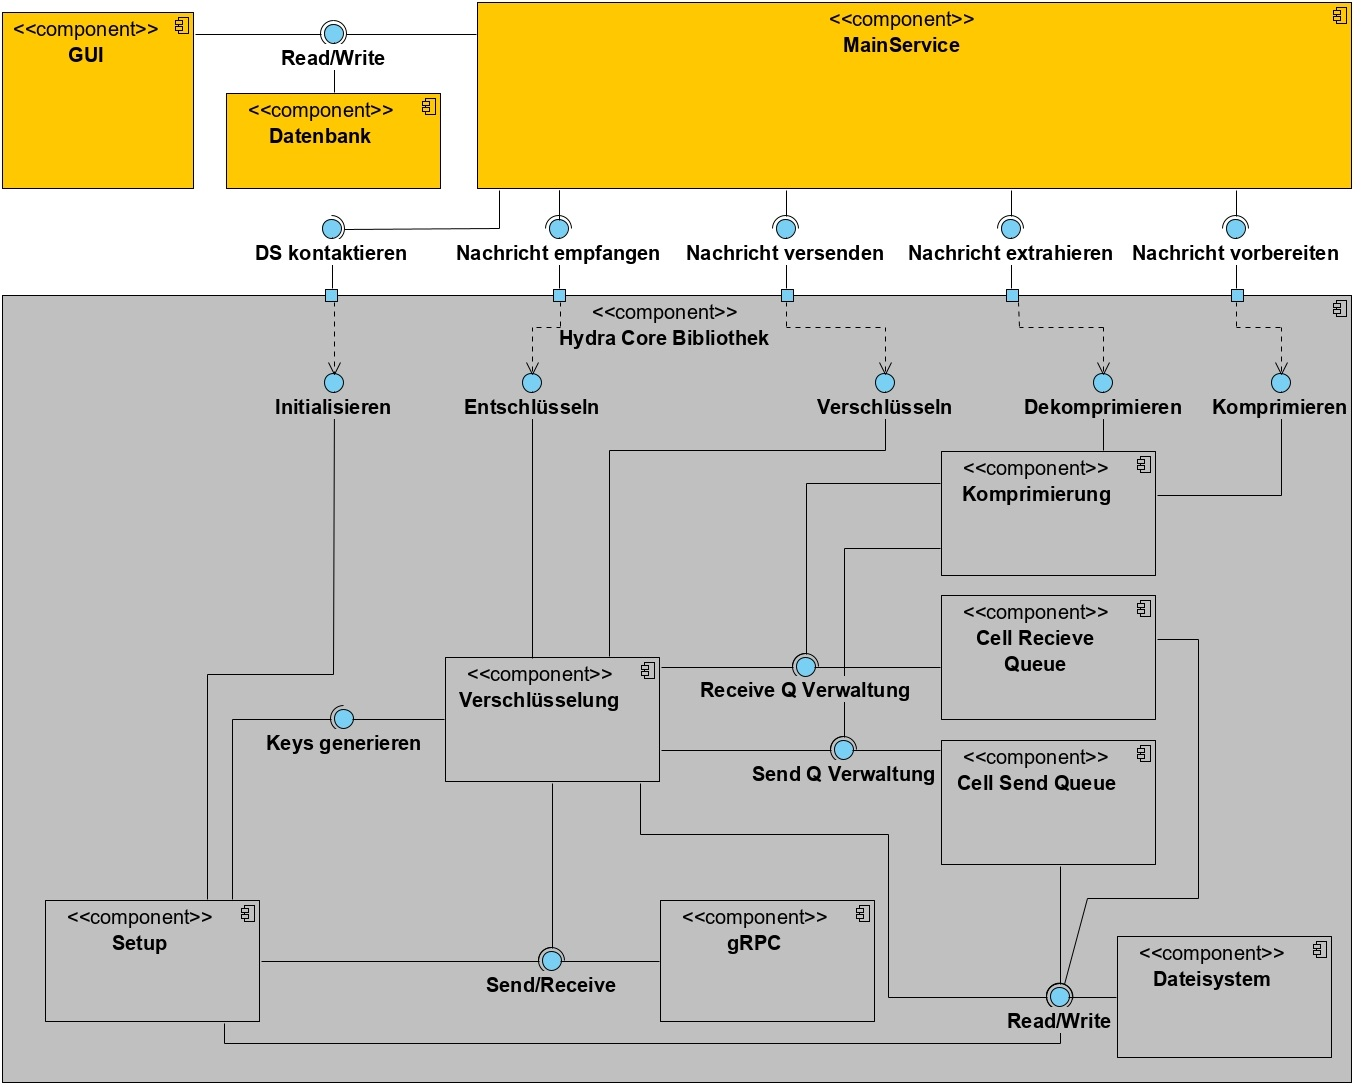
\includegraphics[width=0.9\textwidth]{diagramme/Component_Diagram_E2.jpg}
  \caption{Systemzerlegung des \acp{HC}}
  \label{fig:Bild1}
\end{figure}

\subsubsection{GUI-Activity}
Die \ac{GUI} stellt die Benutzerschnittelle dar, d.h. der Benutzer des \acp{HC} interagiert nur mit der \ac{GUI}. 
Die \ac{GUI} kommuniziert dabei nur mit der Datenbank, indem sie dort Einträge aktualisiert, hinzufügt oder löscht.
Für weitere Informationen siehe Abschnitt \ref{kap2_6:GUI}.

\subsubsection{Hydra Core Bibliothek}
Die \ac{HCB} beinhaltet alle wichtigen Funktionen, welche für das Hydra-Protokoll nötig sind. Sie generiert und verwaltet dabei ihre Daten selbst und kommuniziert mittels \ac{gRPC} mit dem \ac{HS}. Wichtig dabei ist, dass die \ac{HCB} passiv ist, d.h. sie nutzt keine Schnittstellen von anderen Komponenten.\\
\newline
Das Netzwerkinterface \ac{gRPC} bietet eine Schnittstelle für die Netzwerkoperationen senden bzw. empfangen einer Nachricht an. Des Weiteren wird über diese Schnittstelle mit dem \ac{DS} kommuniziert.\\
\newline
Das Dateisystem bietet eine Schnittelle für Lese- und Schreibzugriffe auf persistente Daten an.\\
\newline
Das Setup verbindet sich über \ac{gRPC} mit dem \ac{DS}, ruft die neuen Netzwerkinformationen (siehe Pflichtenheft Kapitel 4.2 /F0510/) von diesem ab und aktualisiert die im Dateisystem vorhandenen Daten. Des Weiteren erstellt das Setup die Setup-Pakete für zukünftige Epochen und versendet diese über \ac{gRPC} an die jeweiligen Mixe.\\
\newline
Bei dem Aufruf \textit{Nachricht vorbereiten} übergibt der \ac{MS} die vorzubereitende Nachricht an die Komprimierung. Diese komprimiert die übergebene Nachricht, indem sie die Textcodierung von UTF-16 in ASCII umwandelt, und gibt sie an die \ac{CSQ} weiter.
Bei dem Aufruf \textit{Nachricht extrahieren} entnimmt die Komponente eine Nachricht aus der \ac{CSQ}, dekomprimiert diese und gibt sie als Rückgabewert an den \ac{MS} zurück.\\
\newline
Die \ac{CSQ} nimmt eine komprimierte Nachricht der Komprimierung entgegen, reiht diese in die Warteschlange hinten ein und legt sie im Dateisystem ab. Auf Anfrage der Komponente Verschlüsselung nimmt die \ac{CSQ} die vorderste Nachricht der Warteschlange, übergibt diese der Verschlüsselung und löscht sie aus dem Dateisystem.\\
Die \ac{CSQ} übernimmt die Fragmentierung für Nachrichten, die für ein einzelnes Paket zu groß wären, reiht die einzelnen Fragmente korrekt in die Warteschlange ein und legt die Fragmente im Dateisystem ab. \\
Außerdem kümmert sie sich um die Zustellungsgarantie von Nachrichten. Sowohl die Zustellungsgarantie als auch die Fragmentierung werden nach TCP-Vorbild implementiert.\\
\newline

Die \ac{CRQ} nimmt ein Datenpaket der Verschlüsselung entgegen und legt dieses im Dateisystem ab. Handelt es sich bei dem Datenpaket um ein Fragment einer größeren Nachricht, so wird die \ac{CRQ} diese zu einer vollständigen Nachricht zusammensetzen, bevor die vollständige Nachricht an die Komprimierung weitergegeben werden kann.\\
\newline
Die Komponente Verschlüsselung generiert auf Anfrage die Schlüssel für das Setup.\\
Des Weiteren verschlüsselt sie Nachrichten mithilfe von \ac{AES} Ende-zu-Ende und generiert aus der verschlüsselten Nachricht eine \ac{CC}. Der Payload der \ac{CC} wird onion-encryptet mithilfe von einem Feistel-Netzwerk mit 12 Runden Threefish-1024.\\
Außerdem kann die Komponente sowohl die \ac{OE} als auch die \ac{E2EE} entfernen.
Die Komponente sendet bzw. empfängt \acp{CC} über \ac{gRPC}. Sie erkennt dabei auch manipulierte \acp{CC} bzw. \acp{DP} und verwirft diese. Ansonsten wird der Inhalt der \acp{CC} an die \ac{CRQ} übermittelt.
Bei dem Aufruf \textit{Nachricht empfangen} gibt die Komponente zurück, ob es eine vollständige Nachricht, ein Fragment oder eine ungültige Nachricht empfangen hat.

\subsubsection{Main-Service}
Der \ac{MS} ist für die Steuerung der Programmabläufe verantwortlich. Somit hat er insgesamt drei Schnittstellen:
\begin{itemize}
\item[1)]Der \ac{MS} kommuniziert mit der Datenbank und kann so indirekt Informationen mit der \ac{GUI} austauschen.
\item[2)]Der \ac{MS} kommuniziert mithilfe des \acp{NDK} mit der \ac{HCB} über einfache, synchrone Methodenaufrufe.
\end{itemize}
Als einzige Komponente kann der \ac{MS} sowohl mit der \ac{GUI} als auch mit der \ac{HCB} kommunizieren.